\documentclass[UTF8,a4paper,11pt,openany]{ctexrep}

\usepackage{geometry}
\usepackage{graphicx}
\usepackage{booktabs}
\usepackage{longtable}
\usepackage{tabularx}
\usepackage{array}
\usepackage{amsmath}
\usepackage{siunitx}
\usepackage{float}
\usepackage{caption}
\usepackage{xcolor}
\usepackage{hyperref}
\usepackage{tikz}
\usetikzlibrary{arrows.meta,positioning,fit,calc,shapes.geometric,backgrounds}

\geometry{left=2.25cm,right=2.25cm,top=2.45cm,bottom=2.35cm}
\setlength{\emergencystretch}{3em}
\renewcommand{\arraystretch}{1.28}
\setlength{\leftmargini}{2em}
\setlength{\leftmarginii}{1.8em}

\definecolor{dmxblue}{HTML}{175A87}
\definecolor{dmxcyan}{HTML}{DDEFF5}
\definecolor{dmxgreen}{HTML}{2E7D5B}
\definecolor{dmxgreenlight}{HTML}{E1F1E8}
\definecolor{dmxyellow}{HTML}{FFF1C7}
\definecolor{dmxred}{HTML}{A63D40}
\definecolor{dmxredlight}{HTML}{F8E3E3}
\definecolor{dmxgray}{HTML}{505A62}
\definecolor{dmxlightgray}{HTML}{F2F4F5}
\definecolor{dmxdark}{HTML}{24313A}

\hypersetup{
  colorlinks=true,
  linkcolor=dmxblue,
  urlcolor=dmxblue,
  pdfauthor={DMX项目组},
  pdftitle={DMX说明文档},
  pdfsubject={DMX低空小目标全景监测系统技术说明}
}

\pagestyle{plain}

\ExplSyntaxOn
\NewDocumentCommand{\pathtext}{m}
  {
    \group_begin:
    \ttfamily
    \exp_args:Ne \tl_map_inline:nn { \tl_to_str:n {#1} }
      { ##1\allowbreak }
    \group_end:
  }
\ExplSyntaxOff
\newcommand{\metricA}{\textcolor{dmxgreen}{\textbf{A--日志实测}}}
\newcommand{\metricB}{\textcolor{dmxblue}{\textbf{B--受控样本}}}
\newcommand{\metricC}{\textcolor{orange!80!black}{\textbf{C--外场经验}}}
\newcommand{\metricD}{\textcolor{dmxred}{\textbf{D--待验证}}}
\newcommand{\yes}{\textcolor{dmxgreen}{\textbf{已完成}}}
\newcommand{\partialdone}{\textcolor{orange!80!black}{\textbf{部分完成}}}
\newcommand{\todo}{\textcolor{dmxred}{\textbf{待完成}}}

\tikzset{
  dmxbox/.style={draw=dmxblue,very thick,rounded corners=2pt,fill=dmxcyan,
                 align=center,minimum height=11mm,text width=31mm,font=\small},
  hwbox/.style={draw=dmxgreen,very thick,rounded corners=2pt,fill=dmxgreenlight,
                align=center,minimum height=13mm,text width=34mm,font=\small},
  storebox/.style={draw=dmxgray,very thick,rounded corners=2pt,fill=dmxlightgray,
                   align=center,minimum height=12mm,text width=36mm,font=\small},
  warnbox/.style={draw=dmxred,very thick,rounded corners=2pt,fill=dmxredlight,
                  align=center,minimum height=12mm,text width=36mm,font=\small},
  layerbox/.style={draw=dmxblue,thick,rounded corners=2pt,fill=white,
                   align=center,minimum height=10mm,text width=35mm,font=\small},
  groupbox/.style={draw=dmxgray,dashed,rounded corners=3pt,inner sep=5pt},
  flow/.style={-{Stealth[length=2.6mm]},very thick,draw=dmxdark},
  dataflow/.style={-{Stealth[length=2.6mm]},very thick,draw=dmxblue},
  controlflow/.style={-{Stealth[length=2.6mm]},very thick,draw=dmxred},
  auxflow/.style={-{Stealth[length=2.3mm]},thick,dashed,draw=dmxgray},
  flowlabel/.style={font=\scriptsize,fill=white,inner sep=1.5pt,align=center},
  decision/.style={diamond,draw=dmxred,very thick,fill=dmxyellow,aspect=2.25,
                   align=center,text width=27mm,inner sep=1.2pt,font=\scriptsize}
}

\begin{document}
\hypersetup{pageanchor=false}

\begin{titlepage}
  \centering
  \vspace*{1.6cm}
  {\fontsize{28}{34}\selectfont\bfseries DMX\par}
  \vspace{0.45cm}
  {\fontsize{21}{27}\selectfont\bfseries 低空小目标全景监测系统\par}
  \vspace{1.2cm}
  {\fontsize{25}{32}\selectfont\bfseries DMX说明文档\par}
  \vspace{0.55cm}
  {\Large 软件、硬件、算法与量化指标技术说明\par}
  \vspace{1.5cm}

  \begin{tabular}{>{\bfseries}r l}
    文档编号： & DMX-HO-001 \\
    文档版本： & V1.3 \\
    编制日期： & 2026年8月26日 \\
    适用工程： & \pathtext{/home/sht/work/DMX_qt} \\
    适用对象： & DMX项目新接手开发、算法和现场维护人员 \\
    文档属性： & 内部技术资料 \\
  \end{tabular}

  \vfill
  \fcolorbox{dmxred}{dmxredlight}{%
    \parbox{0.86\textwidth}{\small
      \textbf{重要说明：}本文把指标分为日志实测、受控样本结果、外场经验和待验证目标。
      当前系统不具备物理测距能力，300--500米为已有外场经验范围，不是未经条件限定的合同保证值；
      DMX Test当前模型\texttt{weights5}已提供训练验证曲线和mAP，但该结果只代表现有验证集上的检测器指标，
      不能替代DMX端到端外场精度，也不能把单帧置信度当作精确率、召回率或mAP。
    }}
  \vspace{1cm}
\end{titlepage}

\pagenumbering{Roman}
\hypersetup{pageanchor=true}

\chapter*{文档控制}
\addcontentsline{toc}{chapter}{文档控制}

\section*{修订记录}
\begin{table}[H]
  \centering
  \begin{tabularx}{\textwidth}{p{1.8cm}p{2.5cm}X p{2.7cm}}
    \toprule
    版本 & 日期 & 修订内容 & 编制/审核 \\
    \midrule
    V1.0 & 2026-08-25 & 建立软硬件总框架、算法说明、量化指标、风险和后续改进路线 & DMX项目组/待审核 \\
    V1.1 & 2026-08-26 & 补充weights5验证指标与曲线、相机系列接口、VT-DT05转台参数及UDP端口职责 & DMX项目组/待审核 \\
    V1.2 & 2026-08-26 & DMX Test切换weights5，并关闭电线杆运行时静态抑制 & DMX项目组/待审核 \\
    V1.3 & 2026-08-26 & 更新当前目标识别详细流程、流程图及手动误检软反馈闭环 & DMX项目组/待审核 \\
    \bottomrule
  \end{tabularx}
\end{table}

\section*{指标证据等级}
\begin{table}[H]
  \centering
  \begin{tabularx}{\textwidth}{p{2.8cm}X p{4.1cm}}
    \toprule
    等级 & 定义 & 使用要求 \\
    \midrule
    \metricA & 从程序日志、文件计数或可重复命令直接统计 & 可作为当前工作站基准，但需保留日志和版本 \\
    \metricB & 在已知图片、人工确认序列或小规模受控回放上验证 & 只能说明该样本结果，不能外推总体准确率 \\
    \metricC & 来自现场观察或项目人员经验，缺少严格距离分桶和标注统计 & 必须写明环境条件，不可直接作为验收承诺 \\
    \metricD & 目标值、待补测值或当前缺失的统计项 & 交付前必须补充测试方案和结果 \\
    \bottomrule
  \end{tabularx}
\end{table}

\tableofcontents
\clearpage
\pagenumbering{arabic}

\chapter{项目概述}

\section{系统定位}

DMX是一套面向低空小目标的\textbf{光学全景监测系统}。系统接收彩色RGB和黑白BW两路
4096$\times$4096图像，结合旋转转台角度形成360度全景，在主控计算机上完成实时显示、
数据记录、疑似目标检测、类别判断、事件去重和极坐标态势显示。

典型目标包括无人机、飞鸟、民航客机以及其他需要人工复核的低空目标。当前系统输出的是
光学方位、全景高度、类别、模型置信度和显示状态，不输出真实距离、海拔、GPS坐标或速度。

\section{项目边界}

\begin{itemize}
  \item “目标雷达”是全景光学图像的极坐标可视化，不是主动电磁雷达。
  \item 极坐标半径由全景图纵坐标映射，不表示米或公里。
  \item 系统没有物理测距传感器，识别距离依赖镜头、目标尺度、天气、光照、姿态和背景对比度。
  \item 单次模型命中可能误报或漏报，工程使用必须结合ROI、连续多圈结果和人工复核。
  \item 正式版和测试版共用大量代码，但控制对象、模型和已启用算法不同，不能混用。
\end{itemize}

\section{当前版本边界}

\begin{table}[H]
  \centering
  \small
  \begin{tabularx}{\textwidth}{p{3.3cm}XX}
    \toprule
    项目 & 正式DMX & DMX Test \\
    \midrule
    可执行文件 & \pathtext{/home/sht/work/DMX_qt/build_linux/DMX} & \pathtext{/home/sht/work/DMX_qt/build_linux_test/DMX_test} \\
    数据来源 & 真实设备UDP路径、SMB图像和转台角度 & 2026-07-23冻结数据本地UDP回放 \\
    转台控制 & 控制真实转台 & 不控制真实转台，合成8秒/圈角度 \\
    当前已部署模型 & 配置中的旧两类weights2，OpenCV DNN CPU确认 & \pathtext{weights5/weights/best.onnx}三类512硬负样本增强模型，ONNX Runtime CUDA直接检测 \\
    检测通道 & 当前主要BW，传统候选+整圈YOLO确认 & RGB/BW独立全图与天空窗口YOLO，传统算法仅诊断 \\
    目标事件融合 & 基础显示合并 & 周期、角度、高度、形态、外观哈希和类别联合关联 \\
    静态杂波 & 尚未正式启用 & 电线杆规则抑制关闭；weights5加人工负样本软反馈 \\
    雷达背景 & 正式能力以BW为准 & BW、RGB、融合三种背景 \\
    用途 & 现场采集和设备运行 & 算法回归、性能测试和模型迭代 \\
    \bottomrule
  \end{tabularx}
\end{table}

\chapter{软硬件总体结构}

\section{硬件与接口框架}

\begin{figure}[H]
  \centering
  \resizebox{0.98\textwidth}{!}{%
  \begin{tikzpicture}[node distance=9mm and 13mm]
    \node[hwbox,text width=40mm] (camera) {海康机器人GigE线阵相机\\RGB/BW双通道\\具体型号待铭牌确认};
    \node[hwbox,below=18mm of camera,text width=40mm] (turntable) {VT-DT05-SHTWT转台\\360度连续旋转\\角度回传、正交输出};

    \node[hwbox,right=25mm of camera,text width=43mm] (device) {设备控制与共享单元\\设备IP：192.168.4.1\\SMB共享：\texttt{/data}};
    \node[hwbox,right=25mm of turntable,text width=43mm] (ttctl) {转台控制器\\串口9600 bit/s\\当前设备节点\texttt{/dev/ttyUSB0}};

    \node[dmxbox,right=29mm of device,text width=49mm,minimum height=17mm] (io) {主控I/O层\\5001/5002控制，8001通知\\CIFS挂载、串口驱动};
    \node[dmxbox,below=9mm of io,text width=49mm,minimum height=17mm] (app) {DMX Qt/C++主程序\\图像解码、全景、检测\\控制、记录、目标界面};
    \node[dmxbox,below=9mm of app,text width=49mm,minimum height=17mm] (gpu) {算法测试GPU链路\\Python常驻进程\\ONNX Runtime CUDA};

    \node[storebox,right=23mm of io,text width=42mm] (display) {显示器与操作输入\\主界面、全景、ROI\\目标极坐标态势};
    \node[storebox,below=13mm of display,text width=42mm] (disk) {本地4T数据盘\\\texttt{/mnt/dmx4t}\\日志、录制、候选、模型};
    \node[storebox,above=9mm of display,text width=42mm] (host) {当前主控工作站\\i9-14900K / 62 GiB\\RTX 5060 Ti 16 GiB};

    \draw[dataflow] (camera) -- node[flowlabel]{RGB/BW图像生成} (device);
    \draw[dataflow] (device) -- node[flowlabel]{8001路径通知\\SMB图像读取} (io);
    \draw[controlflow,bend left=12] (io) to node[flowlabel]{5001设备命令} (device);
    \draw[controlflow,bend left=12] (device) to node[flowlabel]{5002执行应答} (io);
    \draw[controlflow] (turntable) -- (ttctl);
    \draw[controlflow] (ttctl) -- node[flowlabel]{串口角度/控制} (io);
    \draw[flow] (io) -- (app);
    \draw[auxflow,<->] (app) -- node[flowlabel]{测试版IPC/JSON} (gpu);
    \draw[dataflow] (app) -- (display);
    \draw[dataflow] (app) -- (disk);
    \draw[auxflow] (host) -- (io);

    \begin{scope}[on background layer]
      \node[groupbox,fit=(io)(app)(gpu),label={[font=\bfseries\small]above:主控计算机软件域}] {};
    \end{scope}
  \end{tikzpicture}}
  \caption{DMX硬件、网络、串口和主控计算框架}
  \label{fig:hardware-architecture}
\end{figure}

\section{当前主控计算机配置}

\begin{table}[H]
  \centering
  \begin{tabularx}{\textwidth}{p{3.5cm}X p{3.7cm}}
    \toprule
    项目 & 当前实机配置 & 交接说明 \\
    \midrule
    CPU & Intel Core i9-14900K，24核32线程 & 日志和性能数据均基于该主机 \\
    内存 & 62 GiB可用系统内存，8 GiB交换区 & 建议交付机不低于16 GiB，算法机建议32 GiB以上 \\
    GPU & NVIDIA GeForce RTX 5060 Ti，16311 MiB显存 & 测试版CUDA性能基线，不代表CPU正式版性能 \\
    操作系统 & Ubuntu 24.04.4 LTS x86\_64 & 当前构建和运行环境 \\
    Qt & Qt 5.15.2；构建脚本默认\pathtext{/usr/bin/qmake} & 不要误用环境中其他qmake \\
    本地数据盘 & \pathtext{/dev/sda1}，约3.7 TiB，挂载到\pathtext{/mnt/dmx4t} & 2026-08-25可用约1.4 TiB \\
    设备共享盘 & \pathtext{//192.168.4.1/data}挂载到\pathtext{/mnt/dmx_share} & 约915 GiB，当前可用约701 GiB \\
    有线网口 & \pathtext{eno2}，192.168.4.21/24 & 连接设备隔离网 \\
    串口 & \pathtext{/dev/ttyUSB0}，dialout组 & 转台9600 bit/s \\
    \bottomrule
  \end{tabularx}
\end{table}

\section{相机与转台资料}

现有资料包含海康机器人《网口工业线阵相机用户手册V4.0.1》和
《VT-DT05云台用户手册》。相机文件是产品系列通用手册，不是当前装机型号的技术规格书；
因此表中的相机能力应在读取设备铭牌和MVS设备信息后再次确认，不能据此推定像元尺寸或最高行频。

\begin{table}[H]
  \centering
  \small
  \caption{相机系列已确认接口与能力}
  \begin{tabularx}{\textwidth}{p{3.7cm}X p{4.4cm}}
    \toprule
    项目 & 手册可确认内容 & 工程边界 \\
    \midrule
    相机类型 & 海康机器人网口工业线阵相机，千兆以太网GigE接口 & 当前RGB/BW装机具体型号待铭牌确认 \\
    网络与协议 & 标准RJ45；兼容GigE Vision和GenICam；无中继最长传输距离100 m & 100 m是相机网络链路上限，不是目标识别距离 \\
    图像调节 & 支持自动/手动增益和曝光、LUT、Gamma；彩色系列支持白平衡 & 具体参数范围和功能随型号、固件变化 \\
    电源与I/O & 系列采用12-pin P10接口，提供供电、I/O和串口功能 & 接线前必须按装机型号核对引脚定义 \\
    镜头接口 & 系列覆盖M42和M72，M42可经转接环适配F口、C口等 & 当前镜头接口、焦距、光圈和视场角仍未知 \\
    软件侧成像 & 当前DMX接收RGB/BW两路4096$\times$4096 JPEG图像 & 这是系统输出帧规格，不等于传感器完整技术参数 \\
    \bottomrule
  \end{tabularx}
\end{table}

\begin{table}[H]
  \centering
  \small
  \caption{VT-DT05-SHTWT转台厂家参数}
  \begin{tabularx}{\textwidth}{p{3.5cm}p{4.2cm}p{3.5cm}X}
    \toprule
    项目 & 参数 & 项目 & 参数 \\
    \midrule
    型号 & VT-DT05-SHTWT & 传动方式 & 电机直驱 \\
    方位速度 & 0.01--180$^\circ$/s & 方位范围 & 0--360$^\circ$连续旋转 \\
    重复精度 & $\pm0.1^\circ$ & 角度分辨率 & 0.01$^\circ$ \\
    预置位 & 200个 & 信息回传 & 查询回传 \\
    控制接口 & RS485/RS422 & 协议/地址 & Pelco-D / 1 \\
    通信速率 & 9600 bit/s & 输入电源 & DC24V \\
    工作环境 & -30--+65$^\circ$C，湿度90\%$\pm$3\%，非凝结 & 防护等级 & IP66 \\
    \bottomrule
  \end{tabularx}
\end{table}

转台说明书还规定：支撑结构至少承受云台与负载总重量的2倍；室外架空线缆应配置防雷保护；
防雷接地点到云台接地线之间电阻应小于4~$\Omega$；断电后重新上电应间隔15秒。

\section{仍需补齐的硬件资料}

\begin{itemize}
  \item RGB和BW相机铭牌型号、序列号、固件版本、传感器型号、像元尺寸、光谱响应、曝光范围和最高行频。
  \item 镜头型号、接口、焦距、水平/垂直视场角、光圈、畸变参数和调焦方式。
  \item 转台额定载荷、整机功耗、风载等级和各速度档位的实测周期误差。
  \item 设备控制单元、串口转换器、交换机和线缆的具体型号、接线图及备件清单。
\end{itemize}

\chapter{软件架构与模块职责}

\section{软件分层框架}

\begin{figure}[H]
  \centering
  \resizebox{0.98\textwidth}{!}{%
  \begin{tikzpicture}[node distance=9mm]
    \node[layerbox,text width=143mm,minimum height=16mm] (presentation) {
      \textbf{界面与交互}\\
      \texttt{MainWindow}\quad 全景/ROI/旧雷达\quad 目标列表与极坐标态势\quad 图像查看、缩放与正北显示
    };
    \node[layerbox,below=of presentation,text width=143mm,minimum height=16mm] (dispatch) {
      \textbf{配置、接收与调度}\\
      \texttt{AppConfig}\quad \texttt{VideoThread/VideoWorker}\quad
      \texttt{UdpProtocol/TurntableDriver}\quad \texttt{DirectYoloManager}
    };
    \node[layerbox,below=of dispatch,text width=143mm,minimum height=23mm] (algorithm) {
      \textbf{图像与目标算法}\\
      路径解析/解码/方向统一 $\rightarrow$ 全景缓存与极坐标投影 $\rightarrow$
      天空Mask/传统候选/RGB--BW双通道YOLO\\
      $\rightarrow$ 周扫事件关联、类别投票、稳定目标ID和模型硬负样本治理
    };
    \node[storebox,below=of algorithm,text width=143mm,minimum height=18mm] (infrastructure) {
      \textbf{基础设施与持久化}\\
      UDP/CIFS/Serial\quad \texttt{PanoramaSaver/RawRecorder}\quad
      JSONL/ROI/manifest\quad ONNX/PT/Mask/20260723基准回放
    };

    \node[left=5mm of presentation,font=\bfseries\small,align=right] {表示层};
    \node[left=5mm of dispatch,font=\bfseries\small,align=right] {调度层};
    \node[left=5mm of algorithm,font=\bfseries\small,align=right] {算法层};
    \node[left=5mm of infrastructure,font=\bfseries\small,align=right] {基础设施层};

    \draw[<->,very thick,draw=dmxdark] (presentation) --
      node[flowlabel,right]{操作指令/状态更新} (dispatch);
    \draw[flow] (dispatch) -- node[flowlabel,right]{帧、角度与任务调度} (algorithm);
    \draw[auxflow] (infrastructure) -- node[flowlabel,right]{I/O、模型、数据与日志支撑} (algorithm);
  \end{tikzpicture}}
  \caption{DMX软件四层结构与主依赖方向}
  \label{fig:software-architecture}
\end{figure}

\section{核心文件职责}

\begin{longtable}{p{5.4cm}p{9.2cm}}
  \caption{核心源文件速查}\label{tab:files}\\
  \toprule
  文件/目录 & 主要职责 \\
  \midrule
  \endfirsthead
  \toprule
  文件/目录 & 主要职责 \\
  \midrule
  \endhead
  \pathtext{mainwindow.cpp/.h} & 主窗口、设备运行/停止、页面切换、全景缩略图、检测信号接收和目标雷达联动。 \\
  \pathtext{videothread.cpp/.h} & UDP 8001路径接收、原始日志、图像读取、角度回查、方向变换、全景写入、传统检测和正式YOLO确认。 \\
  \pathtext{panoramacache.cpp/.h} & RGB/BW全景缓存、tile写入、无损全景数据组织。 \\
  \pathtext{panoramasaver.cpp/.h} & 无损TIFF、预览图和保存清单。 \\
  \pathtext{rawrecorder.cpp/.h} & 本机A/B半圈录制及目录滚动。 \\
  \pathtext{turntabledriver.cpp/.h} & 转台串口协议、运行方向、速度、角度回传和正交输出。 \\
  \pathtext{turntablecontroldialog.cpp/.h} & 转台参数和手动调试界面。 \\
  \pathtext{udpprotocol.cpp/.h} & UDP 5001设备命令及5002应答。 \\
  \pathtext{appconfig.cpp/.h} & JSON配置加载、默认值和环境变量覆盖。 \\
  \pathtext{directyolomanager.cpp/.h} & 仅测试版编译，管理Python GPU worker并把检测结果送入Qt。 \\
  \pathtext{tools/dmx_direct_yolo_worker.py} & ONNX Runtime CUDA推理、全图/天空窗口调度、RGB/BW互证和固定杂波验证。 \\
  \pathtext{radar_ui/targetradarwindow.cpp} & 目标事件关联、列表排序、三种背景、极坐标页面状态管理。 \\
  \pathtext{radar_ui/targetradarwidget.cpp} & 扫描线、角度刻度、目标点和正北显示偏移。 \\
  \pathtext{radar_ui/polarpanoramaprojector.cpp} & 全景条到极坐标背景投影。 \\
  \pathtext{dmx_config.json} & 正式运行配置；路径、全景、检测、设备和转台参数。 \\
  \pathtext{run_dmx_test.sh} & 测试版隔离端口、固定8秒回放、weights5模型和检测开关总入口。 \\
  \pathtext{TASK_HANDOFF.md} & 历史开发记录、验证结果、风险和决策背景。 \\
  \bottomrule
\end{longtable}

\chapter{数据链路与运行时序}

\section{设备数据流}

\begin{enumerate}
  \item 主程序通过串口启动转台并等待有效角度回传，建立本次运行零点。
  \item 主程序通过UDP 5001向设备发送运行命令，设备通过UDP 5002应答。
  \item 设备生成RGB/BW图像并保存到\pathtext{//192.168.4.1/data}共享目录。
  \item 设备通过UDP 8001发送图像路径文本，而不是发送完整图像字节。
  \item 主程序收到路径后立即写原始JSONL日志，再解析路径并从\pathtext{/mnt/dmx_share}读取图像。
  \item 根据图像接收时间查询角度历史，分别应用RGB/BW延迟补偿。
  \item 图像统一执行逆时针旋转90度和水平镜像；BW再按既有规则做半圈方位补偿。
  \item 图像写入RGB/BW全景缓存，同时进入显示、录制、保存和检测链路。
\end{enumerate}

\section{网络端口职责}

\begin{table}[H]
  \centering
  \small
  \begin{tabularx}{\textwidth}{p{1.8cm}p{3.8cm}p{4.8cm}X}
    \toprule
    端口 & 方向 & 协议定义 & 当前DMX状态 \\
    \midrule
    UDP 5001 & 主控计算机$\rightarrow$采集设备 & 下发设备打开、关闭、PNG/JPG保存、实时采集和停止等文本命令 & 正式版使用 \\
    UDP 5002 & 采集设备$\rightarrow$主控计算机 & 返回原命令和\texttt{OK}或错误原因 & 正式版绑定监听 \\
    UDP 8001 & 采集设备$\rightarrow$主控计算机 & 文件共享模式下发送RGB/BW图像路径文本 & 当前实时图像主链路，DMX Test改用隔离端口18001 \\
    UDP 8002 & 采集设备$\rightarrow$主控计算机 & 黑白JPG压缩图像分块数据 & 协议已定义，当前程序未绑定和解析 \\
    UDP 8003 & 采集设备$\rightarrow$主控计算机 & 彩色JPG压缩图像分块数据 & 协议已定义，当前程序未绑定和解析 \\
    SMB/CIFS & 主控计算机$\leftarrow$设备共享盘 & \pathtext{//192.168.4.1/data}中的实际图像文件 & 挂载到\pathtext{/mnt/dmx_share}后由8001路径驱动读取 \\
    \bottomrule
  \end{tabularx}
\end{table}

当前程序采用“8001路径通知+SMB文件读取”，不是8002/8003图像分块传输。排障时应分别检查
UDP通知是否到达、共享目录是否已挂载以及通知路径对应文件是否可读。

\section{全景坐标关系}

当前无损全景尺寸为65536$\times$4096，由16个4096像素宽方位分片构成。若全景横坐标为
$x\in[0,65535]$，原始算法方位角可按当前旋转方向和零点标定映射为：

\[
  \theta = \operatorname{normalize}\!\left(360^\circ\frac{x}{65536}+\theta_0\right).
\]

显示正北偏移只用于界面：

\[
  \theta_{display}=\operatorname{normalize}(\theta_{raw}-\theta_{north}).
\]

禁止用显示角覆盖原始角度、manifest角度或目标关联角度。

\section{存储数据}

\begin{table}[H]
  \centering
  \small
  \begin{tabularx}{\textwidth}{p{3.4cm}p{5.8cm}X}
    \toprule
    数据类型 & 当前路径 & 内容 \\
    \midrule
    正式运行日志 & \pathtext{/mnt/dmx4t/data/logs} & 启动、网络、队列、检测、保存和错误日志 \\
    原始UDP日志 & \pathtext{/mnt/dmx4t/data/raw_log} & 每条8001文本、接收时间、发送方和长度 \\
    候选目标 & \pathtext{/mnt/dmx4t/data/candidates} & ROI JPG与\pathtext{manifest.jsonl} \\
    本机录制 & \pathtext{/mnt/dmx4t/data/recordings} & RGB/BW A/B半圈JPG \\
    手动全景 & \pathtext{/mnt/dmx4t/data/saves} & 无损TIFF、preview和manifest \\
    测试输出 & \pathtext{/mnt/dmx4t/data/dmx_test} & 隔离日志、候选、原始日志和运行目录 \\
    基准图像 & \pathtext{/mnt/dmx_share/raw/20260723} & RGB/BW各9711张，共约55 GB \\
    DMX Test已部署模型 & \pathtext{/home/sht/data/低小慢数据/yolo26s/result/jiao/pt/weights5/weights/best.onnx} & 512输入，drone/bird/civilian\_airliners，硬负样本增强版 \\
    人工负样本 & \pathtext{/mnt/dmx4t/data/manual_negative_samples} & 干净ROI、空YOLO标签、manifest及运行时软反馈 \\
    \bottomrule
  \end{tabularx}
\end{table}

\chapter{图像处理与目标识别算法}

\section{总体识别流程}

\begin{figure}[H]
  \centering
  \resizebox{0.96\textwidth}{!}{%
  \begin{tikzpicture}[x=1cm,y=1cm]
    \node[dmxbox,text width=28mm] (input) at (-6.2,0) {8001路径通知\\RGB/BW源图\\4096$\times$4096};
    \node[dmxbox,text width=30mm] (prep) at (-2.0,0) {读取与方向统一\\逆时针90度\\再水平镜像};
    \node[dmxbox,text width=30mm] (coord) at (2.2,0) {角度与全景坐标\\16分片、BW半圈补偿\\65536$\times$4096};
    \node[dmxbox,text width=31mm] (mask) at (6.5,0) {预载RGB/BW天空Mask\\几何清理\\64 px边缘内收};

    \node[dmxbox,text width=31mm] (trad) at (-5.2,-2.7) {BW传统算法旁路\\2倍降采样、背景差\\BlackHat与形态纹理};
    \node[storebox,text width=31mm] (diag) at (-5.2,-5.2) {诊断ROI与日志\\\texttt{DETECT\_AUX ui=0}\\不进入目标雷达};

    \node[dmxbox,text width=31mm] (global) at (0.0,-2.7) {全图YOLO分支\\整帧缩放到512\\近距或较大目标};
    \node[dmxbox,text width=31mm] (local) at (4.3,-2.7) {天空窗口YOLO分支\\640窗口、512步长\\逐窗缩放到512};
    \node[dmxbox,text width=35mm] (nms) at (2.15,-5.2) {weights5三类推理\\天空中心复核\\IoU/中心距离NMS};
    \node[decision] (threshold) at (2.15,-7.7) {单流$\geq0.12$\\或跨流融合后$\geq0.12$？};
    \node[warnbox,text width=28mm] (reject) at (-2.2,-7.7) {拒绝正常上报\\保留性能诊断};
    \node[storebox,text width=34mm] (candidate) at (2.15,-10.1) {每帧最多3个候选\\保存512 ROI与manifest\\发送C++候选信号};
    \node[dmxbox,text width=34mm] (feedback) at (6.4,-10.1) {人工负样本软反馈\\位置、类别、dHash\\降权或过滤};
    \node[dmxbox,text width=36mm] (assoc) at (2.15,-12.7) {目标事件关联\\RGB/BW、跨圈周期\\角度、高度、形态、dHash};
    \node[storebox,text width=34mm] (uiout) at (2.15,-15.1) {稳定ID、类别与评分\\左侧目标列表\\光学极坐标态势};
    \node[storebox,text width=34mm] (manual) at (6.4,-15.1) {右键“标记误检并移除”\\图像+空标签+JSONL\\立即重载反馈};

    \draw[dataflow] (input) -- (prep);
    \draw[dataflow] (prep) -- (coord);
    \draw[dataflow] (coord) -- (mask);
    \draw[auxflow] (mask) -- (trad);
    \draw[auxflow] (trad) -- (diag);
    \draw[flow] (mask.south west) -- (global.north east);
    \draw[flow] (mask) -- (local);
    \draw[flow] (global) -- (nms);
    \draw[flow] (local) -- (nms);
    \draw[flow] (nms) -- (threshold);
    \draw[flow] (threshold) -- node[flowlabel]{是} (candidate);
    \draw[controlflow] (threshold) -- node[flowlabel]{否} (reject);
    \draw[dataflow] (candidate) -- (feedback);
    \draw[flow] (feedback) -- (assoc);
    \draw[flow] (assoc) -- (uiout);
    \draw[controlflow] (uiout) -- (manual);
    \draw[controlflow,bend left=18] (manual) to node[flowlabel]{持久化反馈闭环} (feedback);
  \end{tikzpicture}}
  \caption{DMX Test当前逐帧检测、事件融合与人工误检反馈闭环}
  \label{fig:detection-pipeline}
\end{figure}

图\ref{fig:detection-pipeline}描述的是2026年8月26日之后的\textbf{DMX Test实际启用链路}。
正常目标只由weights5直接YOLO产生；传统算法仍运行，但仅用于诊断、对照和后续算法研究，
不能把传统候选数当作雷达目标数。正式DMX仍采用表1.1所列的旧链路，尚未同步本节全部能力。

\section{逐帧识别详细流程}

\begin{enumerate}
  \item \textbf{接收与调度：}8001端口接收RGB/BW图像路径通知，路径线程按时间和角度把任务分发到两路
  \texttt{VideoWorker}。测试回放以8秒/圈、16组/圈运行，每500 ms输入一组，BW与同序号RGB相差约102 ms。
  \item \textbf{图像方向统一：}C++全景链路和Python直接YOLO均执行逆时针90度旋转后水平镜像；BW再按设备关系做
  180度全景分片补偿。后续检测、ROI、方位角和事件关联统一使用65536$\times$4096全景坐标。
  \item \textbf{天空约束：}测试版启动时分别预载RGB和BW的1/4尺度全景Mask。每个分片取对应Mask切片，
  按源图尺度映射，并执行64 px边缘内收。局部窗口的天空覆盖率必须不低于15\%，全图和局部分支的
  最终检测框中心也必须落在天空Mask内。
  \item \textbf{传统诊断旁路：}当前仅BW参与传统算法，先2倍降采样，再以3次历史观测建立背景，计算局部背景暗差、
  CLAHE、BlackHat、连通域、面积/长宽比/紧致度、中心--环带响应、模板相关性和局部杂波分数。
  候选按全景空间去重后保存并记录为\texttt{DETECT\_AUX ui=0}，不进入目标列表。
  \item \textbf{直接YOLO双分支：}RGB和BW每个输入帧都独立进入常驻Python worker。全图分支把完整4096图缩放到
  512；局部分支按640$\times$640、步长512遍历天空窗口，再缩放到512。模型为weights5，类别为
  \texttt{drone}、\texttt{bird}和\texttt{civilian\_airliners}，ONNX Runtime优先使用CUDA。
  \item \textbf{实时预算：}每帧固定执行1次全图推理；局部窗口按游标轮转。正常总预算240 ms，worker排队超过
  450 ms时切换为120 ms追赶预算。至少完成2个局部窗口后才允许因预算停止，未处理窗口由同流同分片游标留到后续帧。
  \item \textbf{框解析与帧内去重：}weights5按端到端$[x_1,y_1,x_2,y_2,conf,class]$解码；解析下限为0.025。
  全图和局部结果合并后，若IoU不低于配置阈值（当前0.45）或中心距离不超过24 px，则保留高置信框。
  目标尺寸只参与框合法性与后续形态兼容，不作为核心识别权重。
  \item \textbf{单流/跨流判决：}单框原始置信度不低于0.12即可输出；0.05--0.12的框必须找到另一图像通道的
  同类别历史框。互证要求时间差2.5--5.5 s、环形横向差不超过384 px、纵向差不超过256 px，融合置信度
  $c_f=1-(1-c_1)(1-c_2)$仍需达到0.12。每帧最多保留3个输出。
  \item \textbf{候选固化：}输出框中心映射到全景坐标，围绕目标保存无界面标注的512$\times$512 ROI，
  同时写入类别、原始/融合置信度、全景框、ROI框、源帧、耗时和Mask模式等manifest字段，再通过
  \texttt{candidateDetected}信号送回C++主线程。
  \item \textbf{人工负样本软反馈：}候选进入雷达事件前，读取人工误检库中的位置、类别和64位dHash。
  同位置或邻近相似外观候选先降低\texttt{confidence}、\texttt{classConfidence}、\texttt{score}和
  \texttt{imageConfidence}；普通低分候选可在此被过滤，强目标只降权不硬拦截。
  \item \textbf{目标事件融合：}保留下来的候选按RGB/BW帧对、半圈异步关系和约8秒跨圈周期进行关联，联合检查
  环形方位差、全景高度、框面积、长宽比、类别和dHash。同一源帧的独立框禁止合并，避免两个同时出现的目标被折叠。
  \item \textbf{显示与人工闭环：}事件获得稳定ID后进入左侧最多7项的目标列表和极坐标态势。人工右键标记误检时，
  程序先保存干净ROI、同名空YOLO标签和JSONL元数据，成功后才删除事件，并立即重载软反馈库。
\end{enumerate}

\subsection{当前判决条件与工程含义}

\begin{table}[H]
  \centering
  \small
  \begin{tabularx}{\textwidth}{p{3.7cm}p{4.5cm}X}
    \toprule
    环节 & 当前条件 & 工程含义 \\
    \midrule
    模型解析下限 & $\max(0.01,0.05/2)=0.025$ & 只控制解码候选池，不等于最终上报阈值 \\
    单流直接输出 & 原始置信度$\geq0.12$ & RGB或BW单独达到阈值即可上报 \\
    低分跨流互证 & 单流$\geq0.05$且融合后$\geq0.12$ & 仅同类别、邻近全景位置和规定时间差可以互证 \\
    帧内NMS & IoU$\geq0.45$或中心距$\leq24$ px视为重复 & 合并全图/局部重复框；当前为类别无关NMS \\
    每帧输出上限 & 3个 & 按融合后置信度排序，限制界面和存储负载 \\
    手动反馈核心范围 & 横向512 px、纵向256 px & 由$\max(256,W/128)$和$\max(128,H/16)$自适应得到 \\
    相似外观范围 & 核心范围的2倍，dHash距离$\leq12$ & 只在邻近区域使用外观相似度，避免全景范围误伤 \\
    手动反馈权重 & 重复标记增强，最低保留0.18 & 是软降权，不是永久黑名单 \\
    反馈后过滤 & 原始置信度$<0.72$，且调整后置信度$<0.16$或评分$<42$ & 强目标保留通过能力；普通重复误报不再进入雷达 \\
    反馈时间衰减 & 14天内全强度，90天内衰减，之后失效 & 防止环境变化后旧位置长期压制真实目标 \\
    \bottomrule
  \end{tabularx}
\end{table}

\fcolorbox{dmxred}{dmxredlight}{%
  \parbox{0.92\textwidth}{\small
  \textbf{实现核对：}\pathtext{DMX_DIRECT_YOLO_BIRD_RATIO=1.10}目前会传入Python worker，
  但当前直接YOLO代码没有用该参数执行drone/bird比值判决；类别来自weights5端到端输出的类别ID。
  图像对比度和清晰度也只写入性能日志，当前不会据此跳过RGB/BW或动态修改阈值。
  后续修改这两项策略时必须先补测试，不能把配置项存在误认为算法已经生效。
  }}

\section{图像预处理与全景拼接}

\begin{itemize}
  \item 每张源图为4096$\times$4096，程序执行逆时针90度旋转后水平镜像。
  \item 根据角度和延迟补偿确定全景分片，RGB和BW分别写入全景缓存。
  \item BW具有既定的180度方位补偿；修改旋转、镜像或tile顺序时必须同时回归全景和目标方位。
  \item UI缩略全景为8192$\times$240；保存预览宽度8192，不影响65536$\times$4096无损全景。
  \item UI队列允许丢弃旧显示帧以保持实时性，但原始UDP日志和录制链路不应因此丢失。
\end{itemize}

\section{天空区域建模}

天空Mask的目标是排除地面、树线、房屋、杆塔和不规则边缘，降低弱小目标检测的搜索空间。

\begin{enumerate}
  \item 使用前3次同方位观测构建低分辨率全景时序样本。
  \item 合并晴空、云天和高置信天空种子，保留与顶部可靠天空连接的大区域。
  \item 删除孤立碎片、侧向口袋、多段悬空区域和窄颈突出区域。
  \item 对不规则边界做额外收缩，再执行全局边缘内收。
  \item 在线检测时按tile切片并放大到源图坐标。
\end{enumerate}

2026-07-23基准Mask最终覆盖2355014个1/4尺度像素，占16384$\times$1024全景的14.04\%。
原始时序Mask为2744012像素；几何清理和64像素内收在保留5个主要天空连通区的同时，
去除了侧向悬空和多段天空列。测试版预载该Mask，避免首次在线建模约7秒的同步卡顿。

\section{传统候选算法}

传统算法主要用于高灵敏候选召回和诊断：

\begin{itemize}
  \item 灰度化、中值滤波和局部背景估计。
  \item 使用背景减图和BlackHat增强暗小目标。
  \item 在天空Mask内按均值、标准差和阈值系数二值化。
  \item 连通域面积、长宽比、紧致度和线状结构筛选。
  \item 中心--环带暗点扩散响应和高通模板相关性。
  \item 映射到全景坐标后执行环形NMS和空间覆盖选样。
\end{itemize}

正式版中传统候选可进入整圈YOLO确认；DMX Test中传统结果记录为\texttt{DETECT\_AUX ui=0}，
不直接污染目标雷达。

\section{直接YOLO双路径}

DMX Test使用最终三类模型，输入为固定1$\times$3$\times$512$\times$512，输出为
1$\times$300$\times$6的端到端检测结果，类别为\texttt{drone}、\texttt{bird}和
\texttt{civilian\_airliners}。

\begin{itemize}
  \item 全图分支：每帧把4096图缩放到512，用于较近或较大的目标。
  \item 局部分支：在天空Mask内按512步长取640$\times$640原分辨率窗口，再缩放到512模型输入，用于远距离小目标。
  \item 正常每帧推理预算240 ms；排队超过450 ms时使用120 ms追赶预算。
  \item 未处理天空窗口保留轮转游标，后续同方位帧继续处理，避免长期只覆盖固定区域。
  \item 单流高阈值为0.12；0.05--0.12低分结果需要另一通道在时空上互证。
  \item 目标尺寸不作为识别核心权重，只用于框合法性和事件形态兼容检查。
\end{itemize}

\section{RGB/BW互补与目标事件融合}

RGB和BW先独立检测，再在已经完成半圈补偿的全景坐标中融合。当前关联考虑：

\begin{itemize}
  \item 同采集帧对：时间差不超过1.2 s。
  \item 相邻半圈异步配对：时间差约2.5--6.5 s，并检查全景位置和框形态。
  \item 同源跨圈重访：按照约8 s扫描周期，使用周期残差、环形方位差、全景高度、形态和ROI感知哈希。
  \item 同一来源帧的独立框不合并，避免同时出现的两个目标被错误折叠。
  \item 类别冲突通常保持分开；严格对齐的RGB/BW冲突可按更高分类置信度投票。
  \item 合并只完成稳定编号和重复折叠，当前不进行速度预测或轨迹外推。
\end{itemize}

\section{误报治理与人工反馈}

早期模型曾把固定电线杆横担连续识别为无人机，测试版因此实现过保守静态杂波验证。
自2026-08-26切换weights5后，\pathtext{run_dmx_test.sh}显式设置
\pathtext{DMX_STATIC_CLUTTER=0}，以下运行时规则当前\textbf{不参与目标过滤}，仅作为历史实现和回退参考：

\begin{itemize}
  \item 同源、同类别目标保持在全景24$\times$12像素范围。
  \item 64位局部dHash距离不超过12，框面积和长宽比保持兼容。
  \item 至少命中5次、持续24 s，并至少3次发现候选下方竖直支撑结构。
  \item 确认为静态后继续保存ROI和manifest，但不再进入正常目标信号。
  \item 外观发生明显变化时先作为新候选上报，避免真实目标经过固定结构时被永久抑制。
\end{itemize}

当前方案将已复核电线杆ROI作为硬负样本纳入weights5训练，由模型直接区分目标与固定结构。
传统算法保持诊断模式；正常候选仍经过RGB/BW互证和事件去重，但不会再按旧电线杆规则、竖直支撑结构直接隐藏。

\subsection{人工误检负样本与软反馈}

为处理树叶、屋檐和固定结构等仍可能出现的误检，DMX Test增加了人工闭环：

\begin{itemize}
  \item 左侧目标列表右键选择“标记为误检并移除”，先确认源ROI可读并完成文件落盘，再从事件列表和雷达删除。
  \item 固定目录\pathtext{/mnt/dmx4t/data/manual_negative_samples}下，\texttt{images/}保存干净ROI，
  \texttt{labels/}保存同名0字节YOLO标签，\texttt{manifest.jsonl}记录模型、类别、置信度、位置、框和dHash。
  \item 启动时读取最近最多1000条人工记录；新标记成功后立即重载，不需要重启程序。
  \item 反馈只在目标事件入口降权，不修改原始图像、YOLO权重或Python推理结果；被反馈过滤的候选写入
  \texttt{TARGET\_ASSOC manual\_feedback\_drop}日志，便于回溯。
  \item 同一方向出现高置信真实目标时仍可通过；因此该机制不能替代硬负样本增训，也不应改成永久位置屏蔽。
\end{itemize}

\chapter{量化指标与当前能力}

\section{基准数据规模}

\begin{table}[H]
  \centering
  \begin{tabularx}{\textwidth}{p{4.4cm}p{3.5cm}X p{2.7cm}}
    \toprule
    指标 & 当前值 & 说明 & 证据 \\
    \midrule
    2026-07-23 RGB图像 & 9711张 & 序号0--9710连续，4096$\times$4096 & \metricA \\
    2026-07-23 BW图像 & 9711张 & 序号0--9710连续，4096$\times$4096 & \metricA \\
    合计图像 & 19422张，约55 GB & 路径逐条存在，重复报文0，JSON错误0 & \metricA \\
    原始采集墙钟跨度 & 6252.486 s & 15:24:30.822至17:08:43.308，含7次大于2 s停顿 & \metricA \\
    正常阶段每路输入 & 约1.772 frame/s & 平均间隔约564.4 ms & \metricA \\
    BW到同序号RGB间隔 & 中位数102 ms & 测试回放保持该间隔 & \metricA \\
    固定8秒回放 & 每路2 frame/s & 每500 ms一组，每圈16组 & \metricA \\
    全天回放时长 & 4855.5 s & 约1 h 20 min 55.5 s，不带入原始停顿 & \metricA \\
    \bottomrule
  \end{tabularx}
\end{table}

\section{最近完整回放性能基线}

表\ref{tab:latest-performance}来自日志：
\pathtext{/mnt/dmx4t/data/dmx_test/logs/2026-08-18/log_13-44-13.txt}。
该次使用当时的\pathtext{weights最终改版/best.onnx}三类512模型、RTX 5060 Ti、固定8秒/圈，
处理4542张RGB/BW图像。该性能表保留为调度基线，不代表2026-08-26启用的weights5已经完成全量性能回归。

\begin{table}[H]
  \centering
  \small
  \caption{2026-08-18最新运行性能复算}
  \label{tab:latest-performance}
  \begin{tabularx}{\textwidth}{p{4.4cm}rrrrX}
    \toprule
    指标 & 样本数 & 平均 & P50 & P95/最大 & 说明 \\
    \midrule
    全图单次GPU推理 & 283 & 3.37 ms & 3.20 ms & 4.10/4.80 ms & 无局部窗口时的模型推理 \\
    局部窗口活动推理 & 287 & 81.78 ms & 89.10 ms & 105.80/109.00 ms & 同一次调度可处理多个窗口 \\
    图像解码与变换 & 570 & 110.55 ms & 110.10 ms & 127.60/362.70 ms & 共享盘读取、解码和方向处理 \\
    直接YOLO处理总耗时 & 570 & 180.19 ms & 160.20 ms & 241.50/382.90 ms & 不含进入worker前排队 \\
    worker排队时间 & 570 & 53.42 ms & 23.70 ms & 160.20/311.20 ms & 当前未形成持续积压 \\
    排队+处理 & 570 & 233.61 ms & 211.60 ms & 400.90/533.40 ms & 偶发超过500 ms，但未连续增长 \\
    图像处理FPS日志采样 & 2272 & 292.02 ms & 279 ms & 375/634 ms & 每秒聚合采样，不等同单帧精确延迟 \\
    \bottomrule
  \end{tabularx}
\end{table}

本次4542帧回放中未发现\texttt{SEQ gap}、持续解码失败或非零fail；在每路500 ms输入间隔下，
P95排队加处理约400.9 ms，能够跟上固定8秒全景刷新。最大533.4 ms说明仍存在偶发跨周期，
但目前没有形成持续队列增长。该结论属于当前主机和当前数据的性能基线，不应直接外推到其他硬件。

\section{识别效果与精度状态}

\fcolorbox{dmxblue}{dmxcyan}{%
  \parbox{0.92\textwidth}{\small
  \textbf{结论：可以报告weights5检测器的验证集指标，但仍不能给出DMX整机“现场识别准确率”。}
  \texttt{weights5}包含\texttt{results.csv}、PR/F1曲线和混淆矩阵；最佳轮次的
  precision、recall和mAP见表\ref{tab:weights5-metrics}。这些数值依赖当前数据划分、标注质量、
  IoU与置信度设置，不包含共享盘读取、天空Mask、RGB/BW调度、事件融合和外场距离条件。
  2026-07-23全量数据仍未完成逐目标真值标注，因此不能用模型置信度或连续命中次数替代系统精度。
  }}

\clearpage

\begin{table}[H]
  \centering
  \small
  \caption{weights5模型验证结果}
  \label{tab:weights5-metrics}
  \begin{tabularx}{\textwidth}{p{4.2cm}p{3.4cm}X p{2.6cm}}
    \toprule
    指标 & 结果 & 说明 & 证据 \\
    \midrule
    训练记录 & 18个epoch & 配置计划30个epoch、patience=8；结果文件记录至epoch 18 & \metricA \\
    最佳轮次 & epoch 10 & 以验证集mAP50--95最大值选择 & \metricA \\
    Precision / Recall & 90.49\% / 68.79\% & 最佳轮次三类总体框检测指标 & \metricB \\
    mAP50 / mAP50--95 & 78.98\% / 35.61\% & 最佳轮次三类总体指标 & \metricB \\
    各类AP50 & drone 80.9\%；bird 77.1\%；civilian\_airliners 78.9\% & 从最佳权重PR曲线读取 & \metricB \\
    最佳总体F1 & 约0.77 & 曲线对应置信度阈值约0.267，不是固定部署阈值建议 & \metricB \\
    硬负样本留出集 & 12次检测降至0次 & 16张图片、conf=0.30；只证明该小规模受控集合上的下降 & \metricB \\
    候选ONNX & 38,109,876 bytes & SHA-256：\pathtext{e68c15744109f1ec52952001994dc59bddecbfe6df72c9a2932911fbfe8b094f} & \metricA \\
    部署状态 & 已接入DMX Test & 2026-08-26按测试要求启用；正式DMX未更新 & 已确认边界 \\
    \bottomrule
  \end{tabularx}
\end{table}

当前权重来自训练任务\pathtext{XT_yolov26s_s512_hardneg_v2}，输入尺寸512，batch 8，优化器AdamW，
初始学习率0.0002，随机种子20260821，启用AMP和确定性训练。最佳轮次相比最后一轮更优：
最后一轮mAP50为76.74\%、mAP50--95为33.34\%，因此部署时必须选\texttt{best.onnx}而不是\texttt{last.pt}。

\begin{figure}[H]
  \centering
  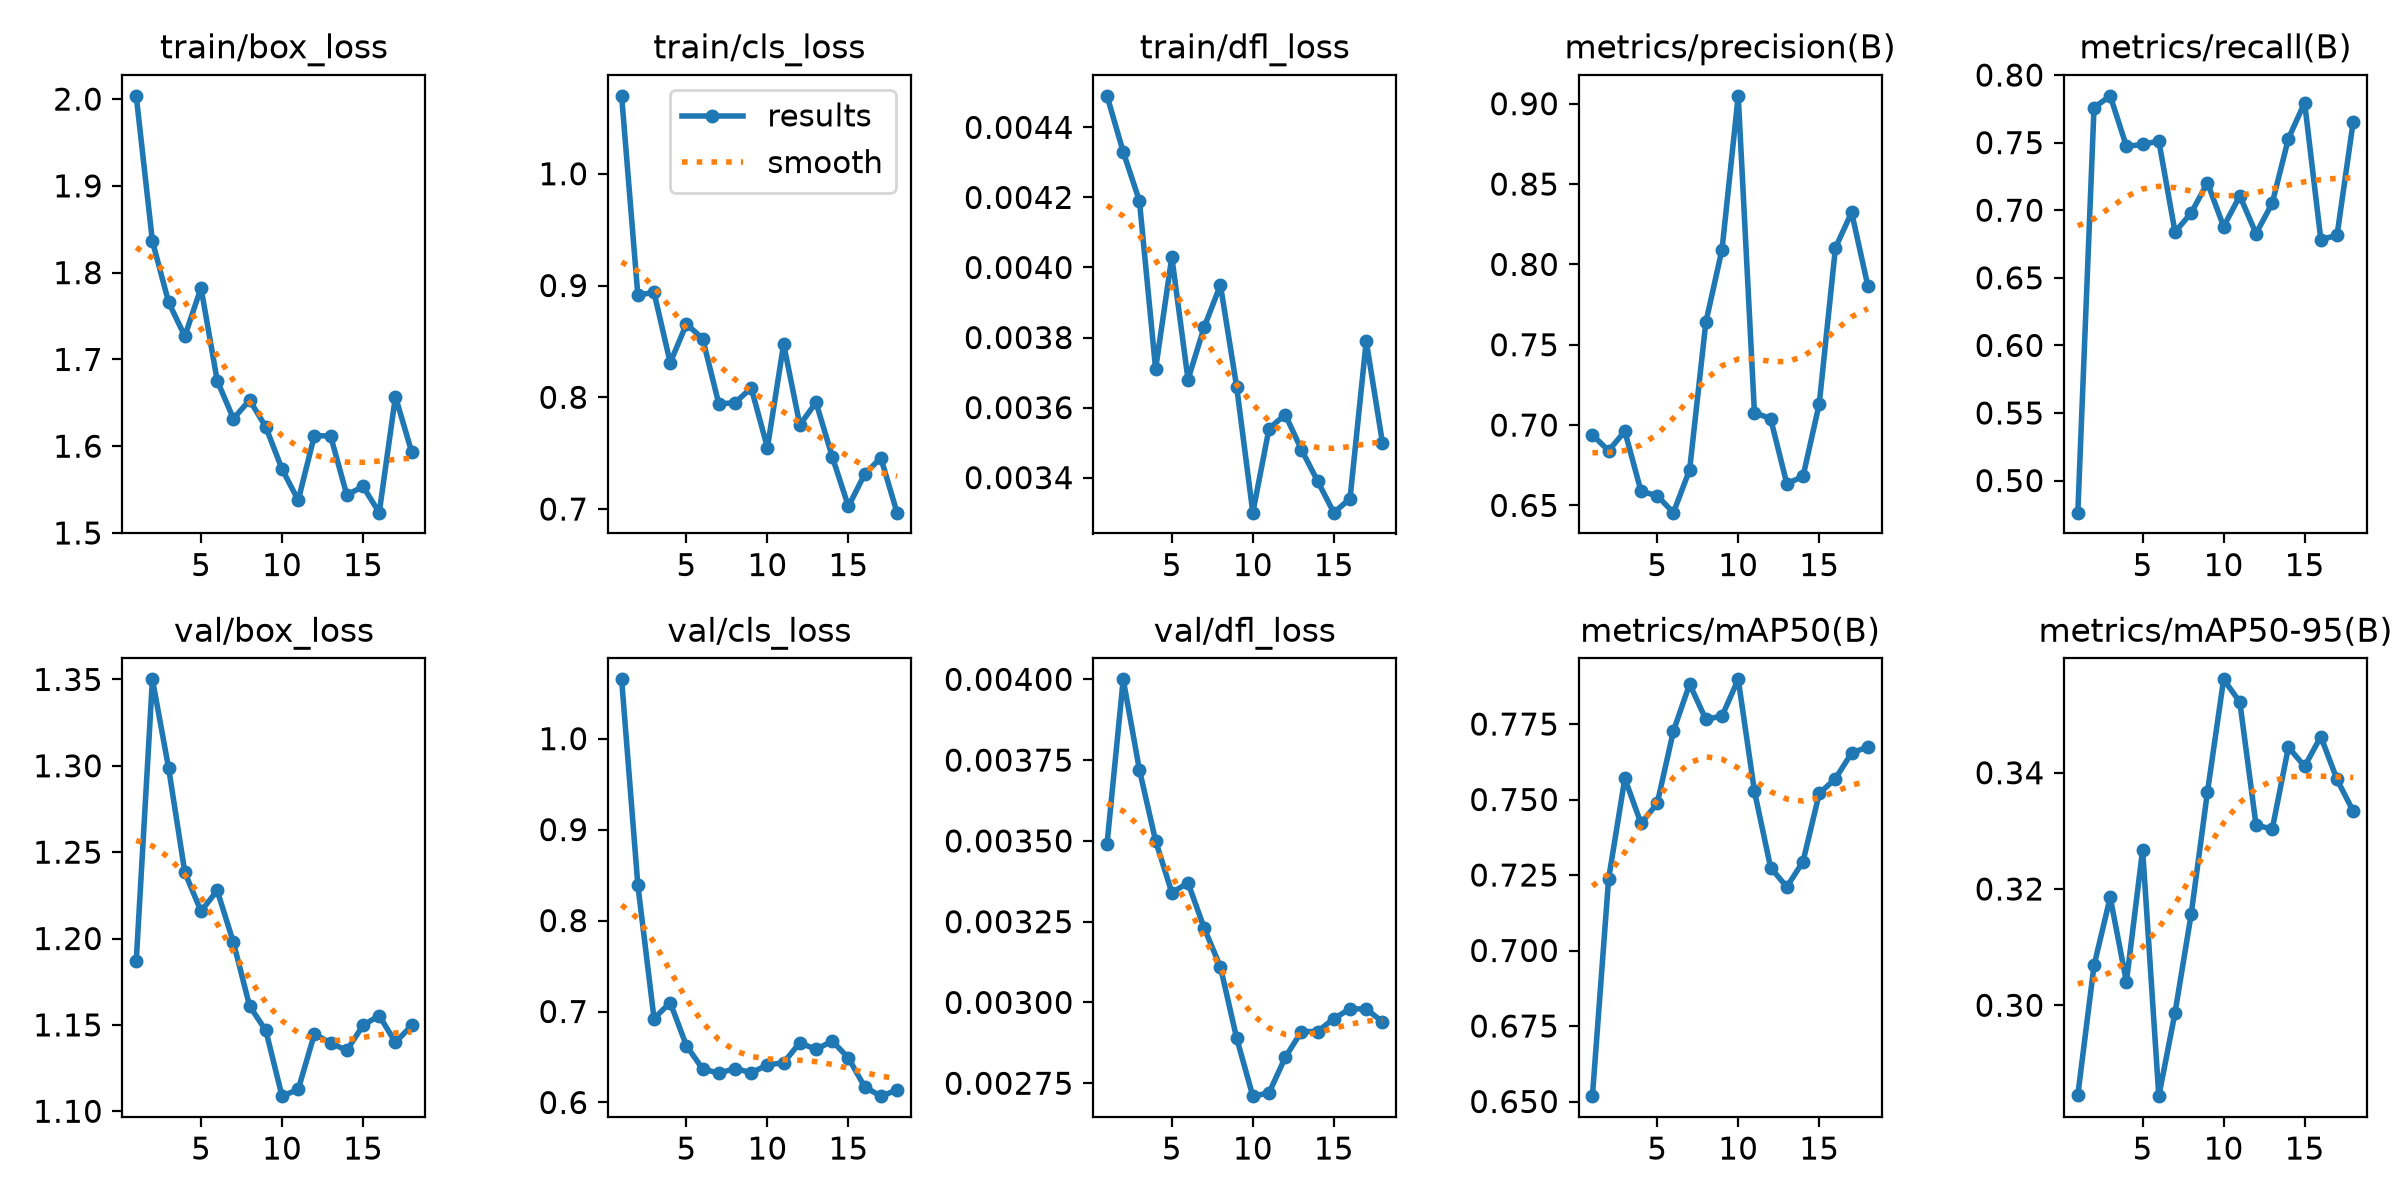
\includegraphics[width=0.98\textwidth]{figures/handover/weights5_results.png}
  \caption{weights5训练损失及验证集Precision、Recall和mAP曲线}
  \label{fig:weights5-results}
\end{figure}

\begin{figure}[H]
  \centering
  \begin{minipage}[t]{0.49\textwidth}
    \centering
    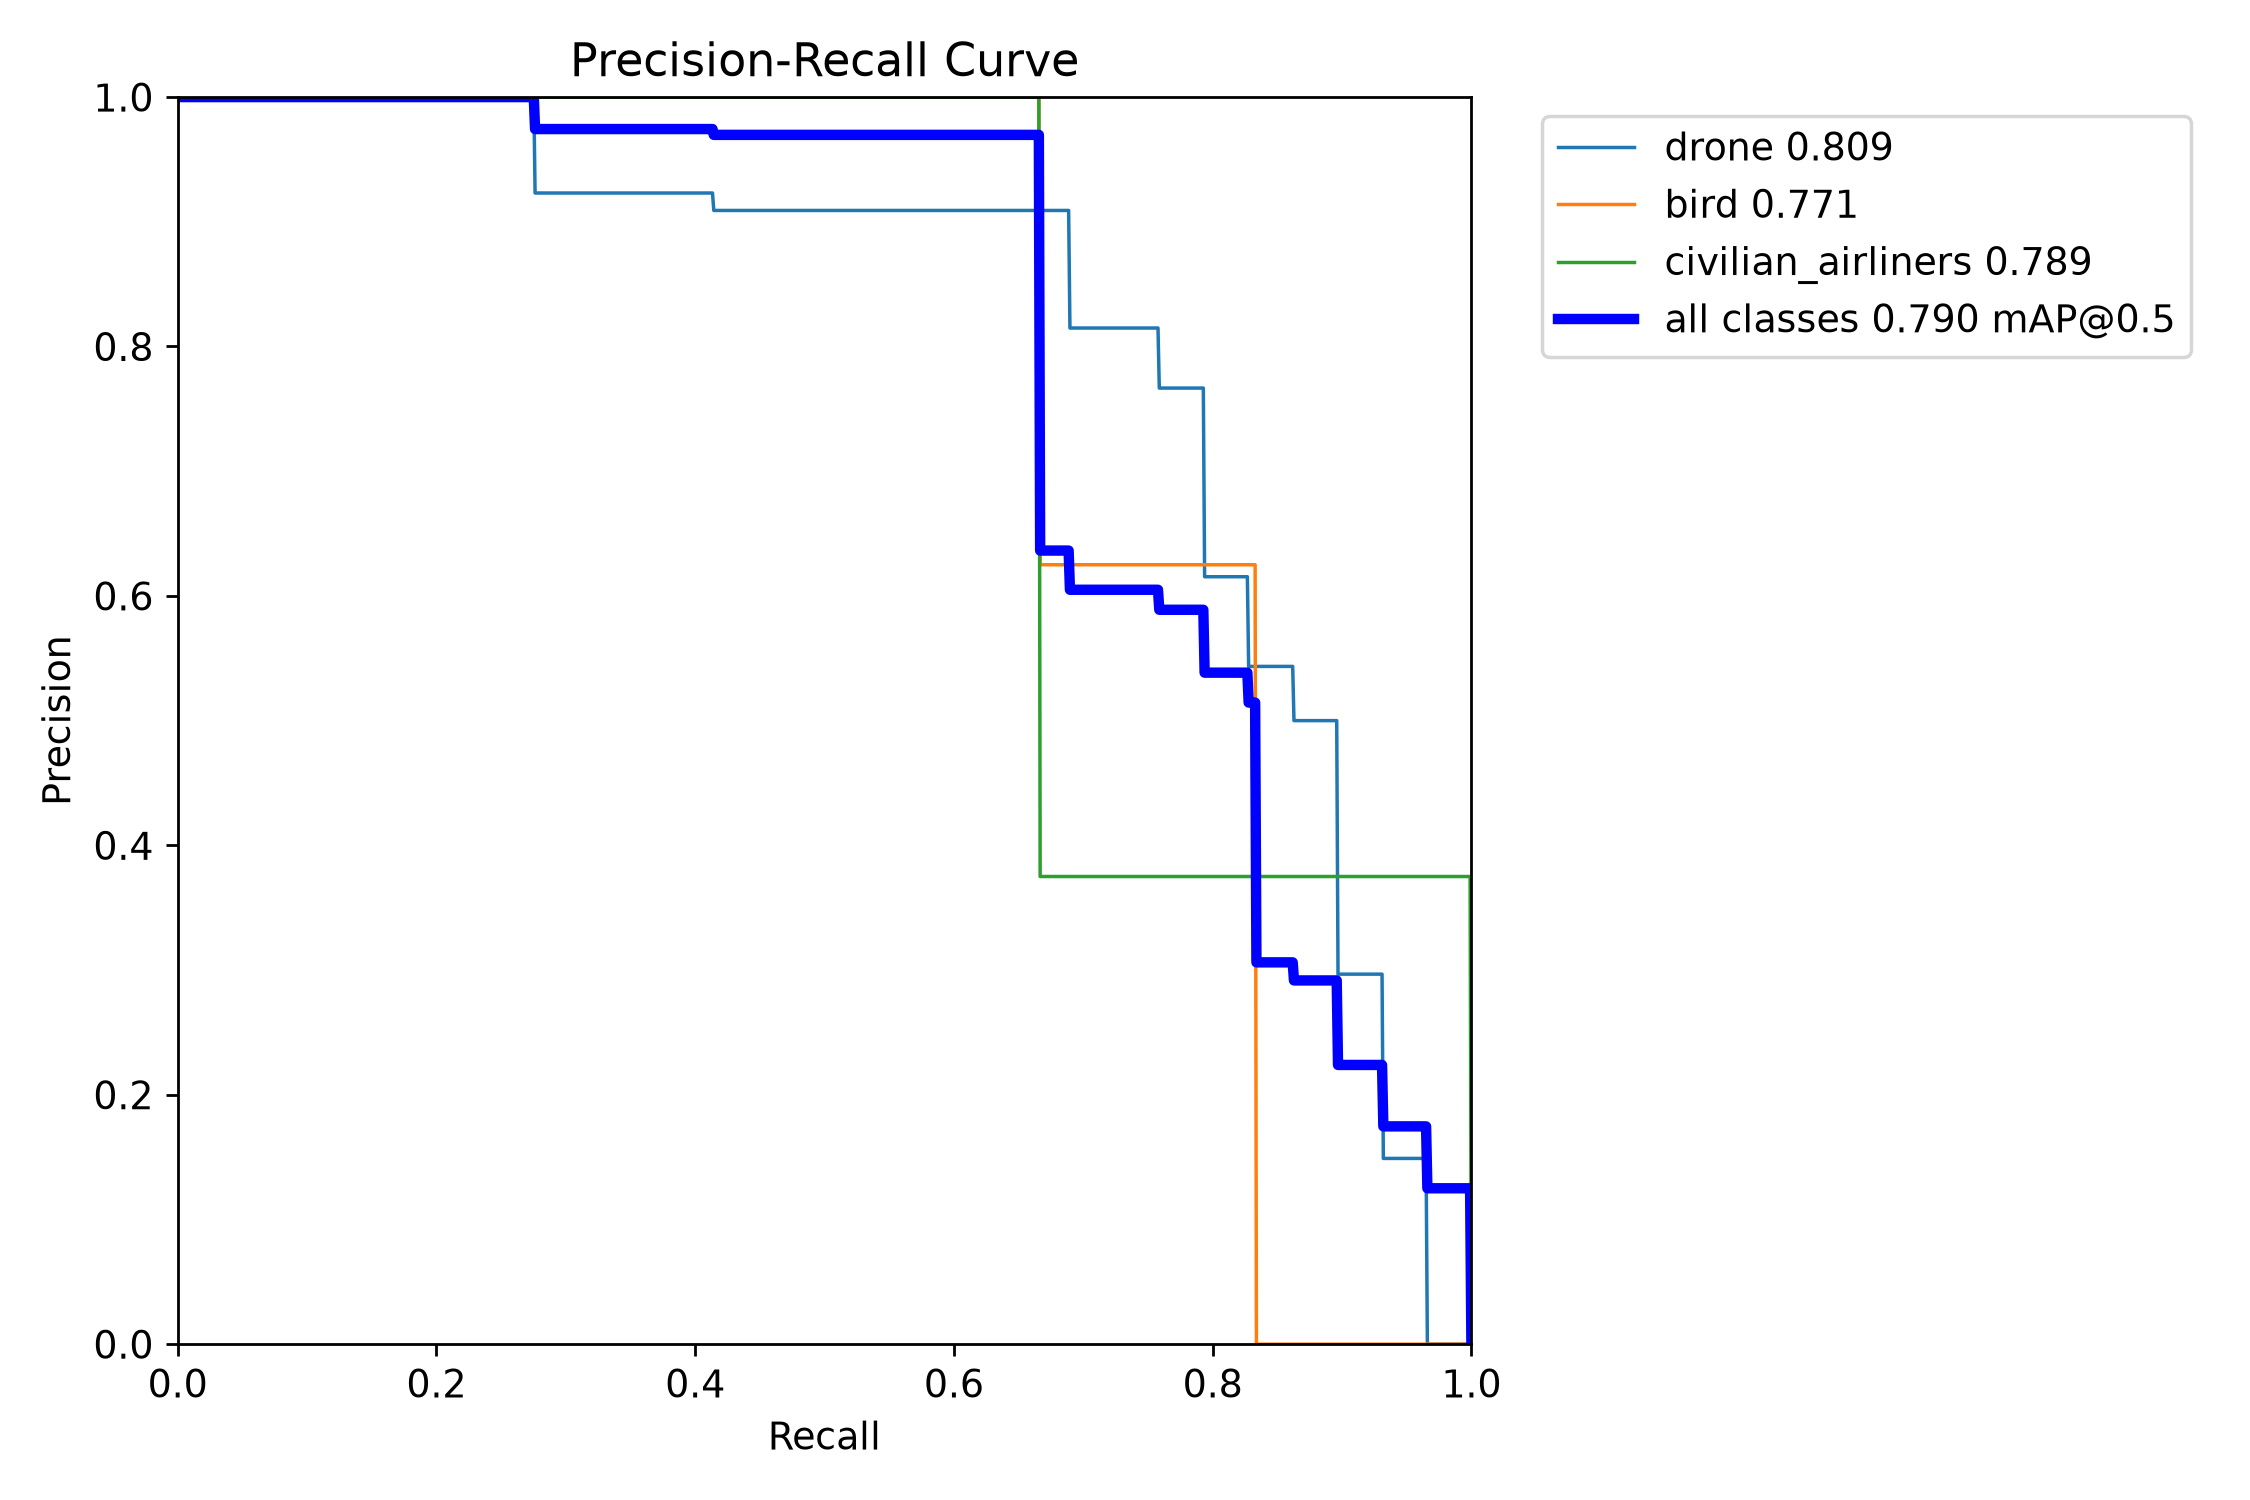
\includegraphics[width=\linewidth]{figures/handover/weights5_pr_curve.png}
  \end{minipage}\hfill
  \begin{minipage}[t]{0.49\textwidth}
    \centering
    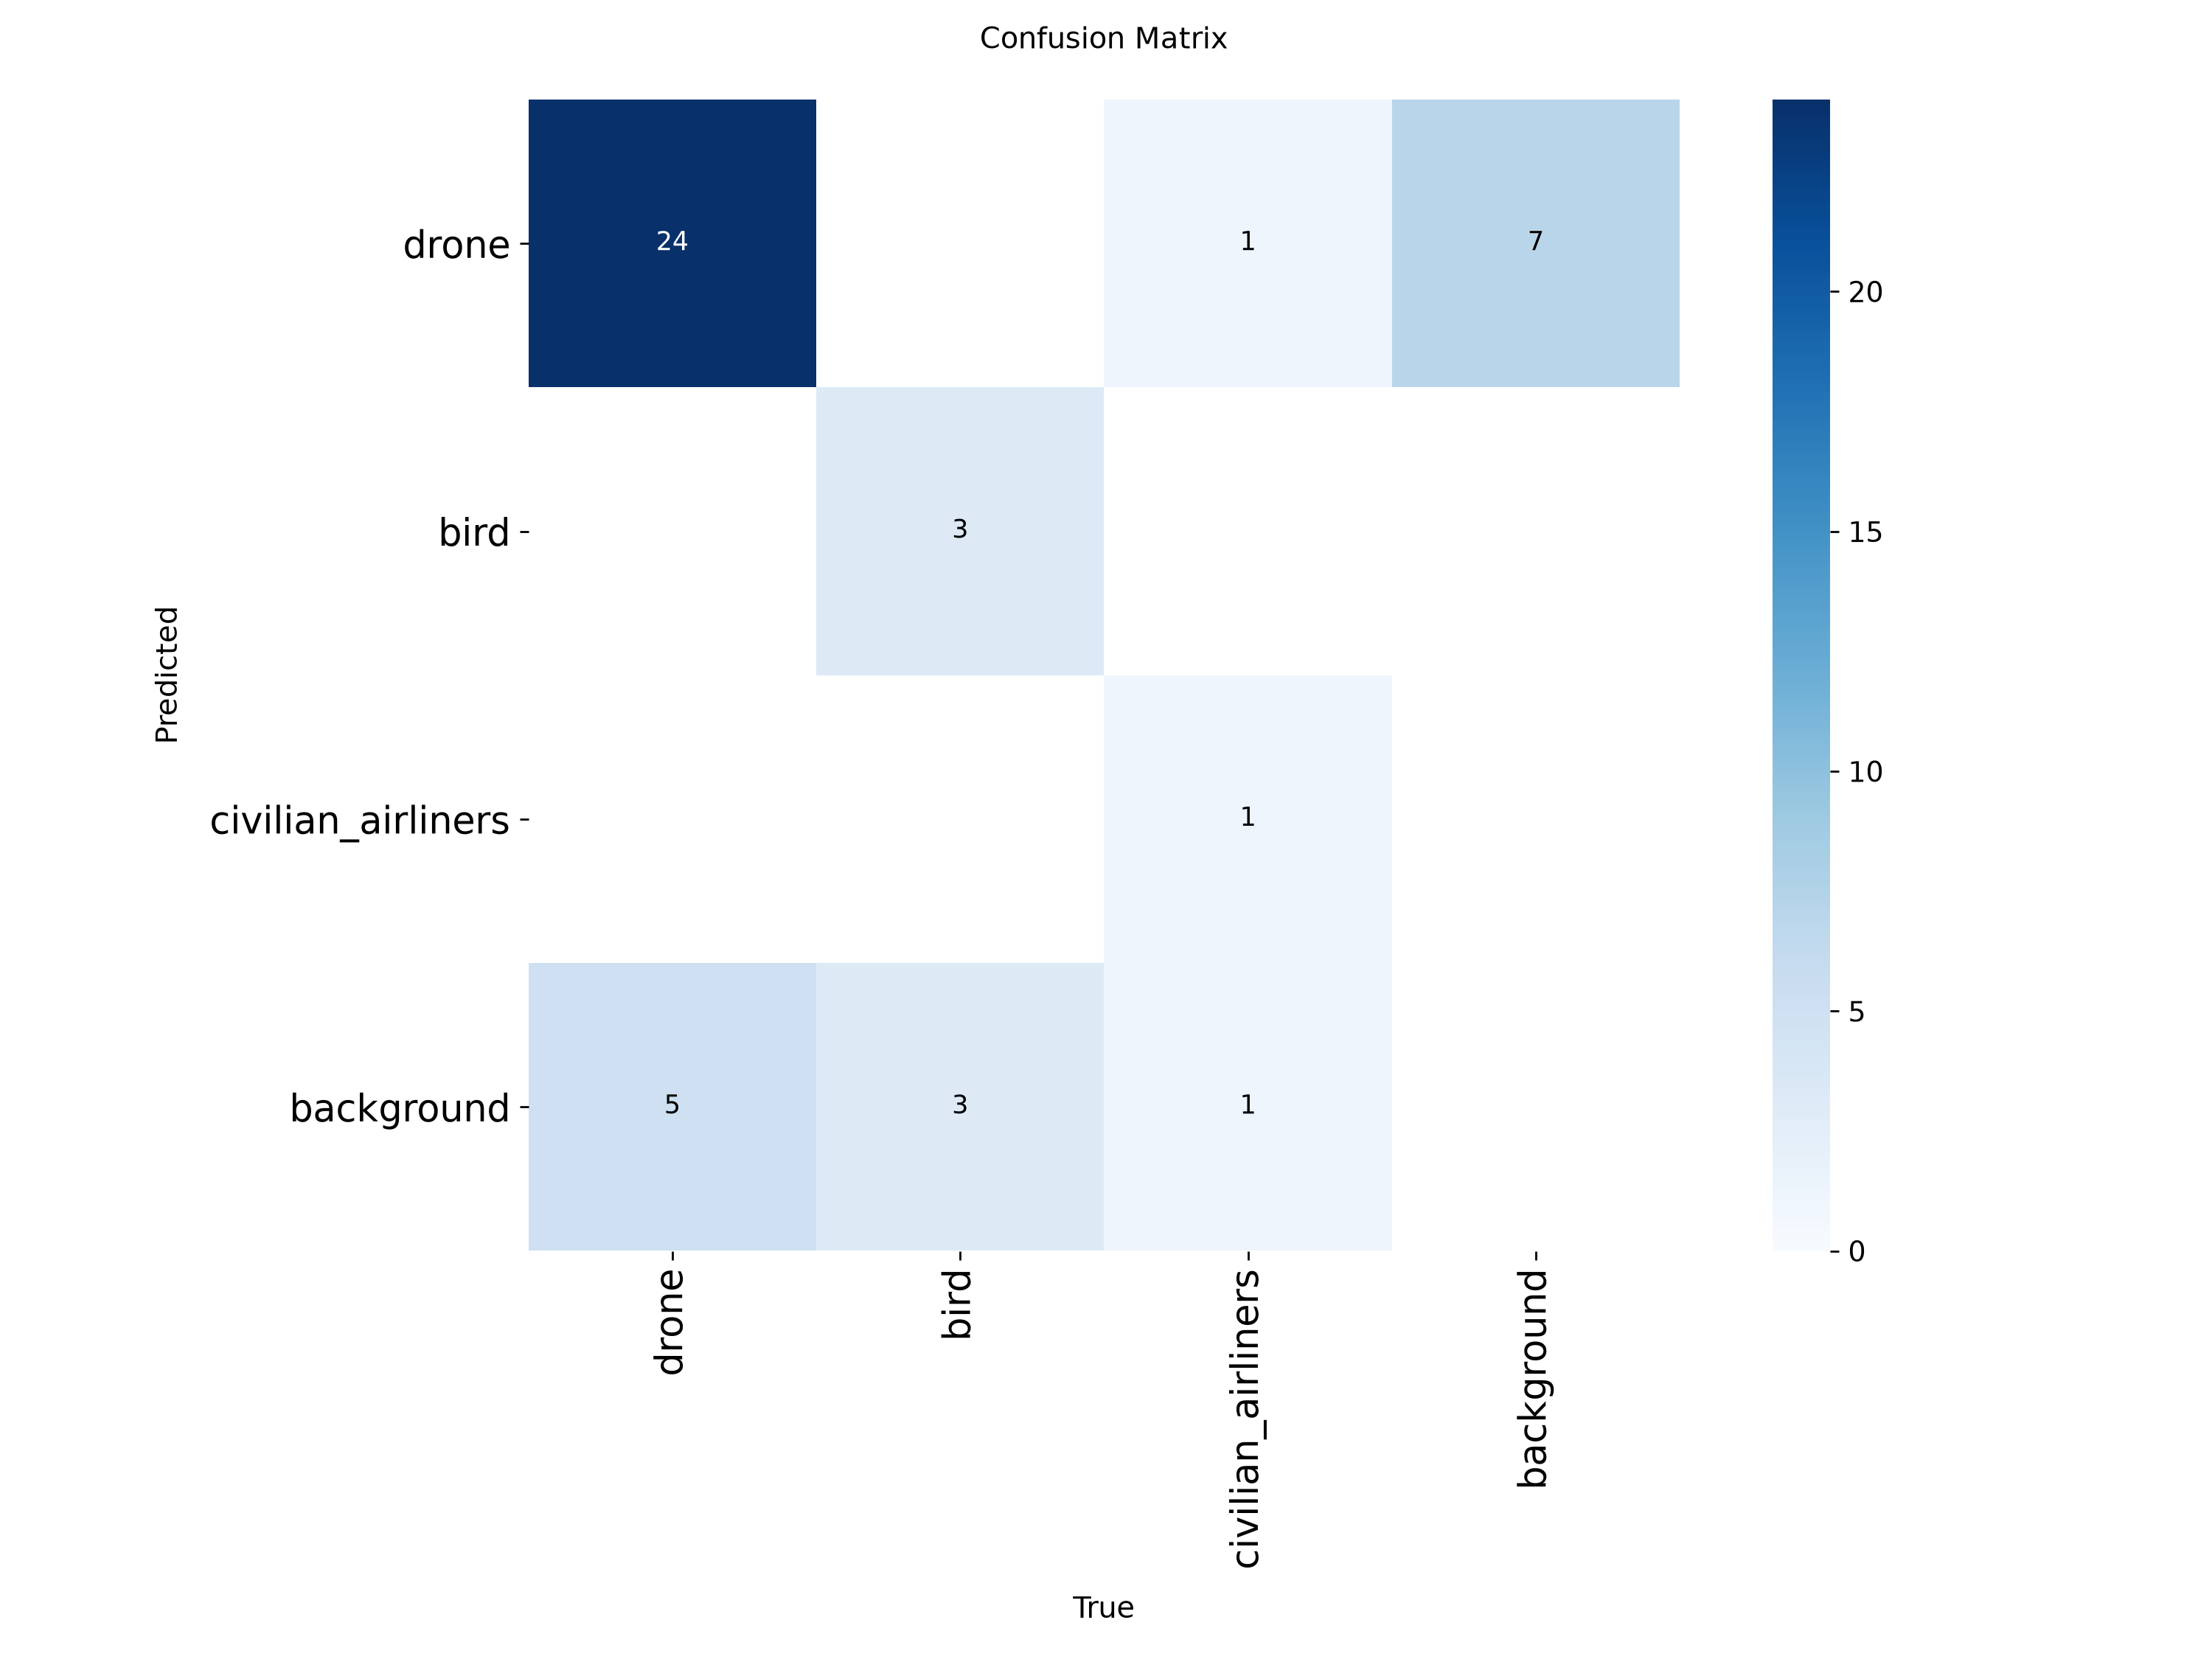
\includegraphics[width=\linewidth]{figures/handover/weights5_confusion_matrix.png}
  \end{minipage}
  \caption{weights5的PR曲线（左）与原始计数混淆矩阵（右）}
  \label{fig:weights5-pr-confusion}
\end{figure}

混淆矩阵只包含38个标注目标（drone 29、bird 6、civilian\_airliners 3），并显示7次背景误检，
类别分布明显不均衡。特别是bird和civilian\_airliners样本量很小，当前每类AP50不宜直接外推到复杂现场。

\begin{table}[H]
  \centering
  \small
  \begin{tabularx}{\textwidth}{p{4.1cm}p{4.0cm}X p{2.6cm}}
    \toprule
    指标 & 当前结果 & 适用边界 & 证据 \\
    \midrule
    无人机已知帧检测 & 类别drone，置信度0.806 & 单个已知样本；置信度不是总体精确率 & \metricB \\
    检测坐标一致性 & 新检测(190,1476)，历史基准(191,1476)，横向差1 px & 单个已知BW帧 & \metricB \\
    飞鸟类别输出 & 已知鸟类帧可输出bird & 只证明类别链路贯通 & \metricB \\
    事件去重冒烟测试 & 47条检测形成33个事件，完成14次合并 & 小规模受控manifest回放 & \metricB \\
    连续跨圈保持 & 同一无人机连续9圈保持一个编号 & 不等于长期跟踪准确率 & \metricB \\
    同帧多目标分离 & 同一帧两只鸟保持两个编号 & 针对已知受控样本 & \metricB \\
    三类候选关联测试 & 106条候选：61次新建、45次合并 & 验证类别约束与RGB/BW合并路径 & \metricB \\
    固定电线杆误报簇 & 人工确认101张唯一误报ROI & 同一根电线杆横担，模型曾连续命中100次 & \metricB \\
    历史静态抑制结果 & 第5次确认静态，后续抑制96次；1次曝光变化保护上报 & 旧规则结果；2026-08-26起已关闭 & \metricB \\
    历史真无人机静态误压 & 受控样本为0 & 旧规则结果；当前不再执行该过滤 & \metricB \\
    DMX端到端Precision/Recall/F1/mAP & 未形成正式统计 & weights5表中数值仅为检测器验证集指标；整机仍需冻结标注回放集 & \metricD \\
    每小时虚警数/每圈漏检数 & 未形成正式统计 & 需要按场景、距离、天气分桶 & \metricD \\
    \bottomrule
  \end{tabularx}
\end{table}

\section{识别距离}

\begin{table}[H]
  \centering
  \begin{tabularx}{\textwidth}{p{4.0cm}p{3.2cm}X p{2.7cm}}
    \toprule
    指标 & 当前量化值 & 条件与解释 & 证据 \\
    \midrule
    小型无人机有效识别距离 & 约300--500 m & 项目外场经验范围；目标可见、天气和对比度较好时，上限可接近500 m & \metricC \\
    可承诺最远距离 & 尚未确定 & 缺少测距真值、目标尺寸分级和多天气重复试验，不能把500 m写成无条件保证值 & \metricD \\
    系统测距输出 & 不支持 & 当前界面径向位置是全景高度，不是距离 & 已确认边界 \\
    模型距离输入/输出 & 不包含 & 最终ONNX导出信息明确\texttt{distance\_output=false} & \metricA \\
    \bottomrule
  \end{tabularx}
\end{table}

300--500 m能力受以下变量共同影响：目标实际翼展和姿态、镜头焦距与调焦、目标像素尺寸、
运动模糊、曝光、云层/树线背景、雨雾、阳光方向和模型训练覆盖。后续应使用激光测距、GPS标定
或已知距离航线，在100 m为一档的距离桶中统计召回率和误报率，形成正式距离曲线。

\section{当前工程能力汇总}

\begin{table}[H]
  \centering
  \small
  \begin{tabularx}{\textwidth}{p{4.1cm}p{3.6cm}X}
    \toprule
    能力 & 当前状态 & 说明 \\
    \midrule
    RGB/BW 360度全景 & \yes & 正式版可用；方向关系不可随意修改 \\
    设备和转台控制 & \yes & UDP 5001/5002、串口9600、角度回传 \\
    原始UDP日志与回放 & \yes & 20260723完整基准已验证 \\
    天空Mask传统候选 & \yes & 正式版和测试版共用基础实现 \\
    weights5三类CUDA模型 & \partialdone & 已同步到DMX Test并通过加载/单帧冒烟，尚未移植正式版 \\
    RGB/BW互补检测 & \partialdone & 测试版可用，正式版待回归 \\
    目标事件去重 & \partialdone & 测试版增强逻辑可用，不是完整追踪 \\
    固定结构误报治理 & \partialdone & weights5已加训硬负样本；运行时位置/dHash/支撑结构抑制已关闭 \\
    RGB/BW融合背景 & \partialdone & 测试版可用，正式版仍以BW为准 \\
    真实距离/速度/轨迹 & \todo & 无测距；当前不做运动模型和轨迹外推 \\
    模型验证报告 & \partialdone & weights5已有总体PR/mAP和混淆矩阵；验证集类别数量偏少且不均衡 \\
    系统精度报告 & \todo & 缺20260723端到端人工真值、每小时虚警、发现延迟和距离分桶 \\
    \bottomrule
  \end{tabularx}
\end{table}

\chapter{构建、启动与现场操作}

\section{正式版构建与启动}

\begin{verbatim}
cd /home/sht/work/DMX_qt
./build_linux.sh
./build_linux/DMX
\end{verbatim}

桌面正式入口为\pathtext{/home/sht/桌面/DMX.desktop}。启动前必须确认：

\begin{verbatim}
ping -c 3 192.168.4.1
findmnt /mnt/dmx_share
findmnt /mnt/dmx4t
test -w /mnt/dmx4t/data && echo writable
ls -l /dev/ttyUSB* /dev/ttyACM* 2>/dev/null
\end{verbatim}

共享盘未挂载时执行：

\begin{verbatim}
cd /home/sht/work/DMX_qt
./mount_share.sh
\end{verbatim}

\section{测试版构建与启动}

\begin{verbatim}
cd /home/sht/work/DMX_qt
./build_test.sh
./run_dmx_test.sh
\end{verbatim}

桌面入口为\pathtext{/home/sht/桌面/dmx_test.desktop}。点击“设备运行”后从当前位置开始固定8秒/圈回放；
“设备停止”只暂停，不清空算法状态。需要从零开始时关闭程序并重新启动。

\section{标准现场启动顺序}

\begin{enumerate}
  \item 检查设备安装、旋转净空、线缆防缠绕、供电和接地。
  \item 检查设备网络、SMB共享、本地4T盘和串口权限。
  \item 启动DMX，打开转台控制，确认串口、9600 bit/s、方向、速度和角度回传。
  \item 人员离开转台旋转区域后，在主界面点击“设备运行”。
  \item 观察角度连续变化、RGB/BW图像更新、全景方向和日志队列。
  \item 检测启用时至少等待3圈背景和天空建模，不要在预热阶段立即调整阈值。
  \item 采集任务中同步保存原始UDP日志、RGB/BW数据、模型版本和现场距离说明。
\end{enumerate}

\section{正常停机}

先停止录制，再点击“设备停止”，确认转台完全停止和正交输出关闭，最后关闭软件。
软件无响应时优先使用设备实体停止或断电措施，转台停止前不得进入旋转范围。

\chapter{已知问题与风险}

\section{算法风险}

\begin{enumerate}
  \item \textbf{模型指标不能代表整机：}weights5已有验证集precision、recall和mAP，但尚无DMX端到端外场精度基线。
  \item \textbf{验证集规模偏小：}混淆矩阵仅含38个目标，其中bird 6个、civilian\_airliners 3个，类别结论方差较大。
  \item \textbf{固定结构误报：}旧模型曾连续命中电线杆横担；weights5在16张留出集上清零，但关闭运行时抑制后仍需扩大独立场景验证。
  \item \textbf{天空边界权衡：}内收过小会引入树叶和建筑边缘，内收过大会漏掉贴近地平线的真目标。
  \item \textbf{RGB/BW分类差异：}不同成像通道可能对同一目标输出不同类别，需要保留来源和置信度审计。
  \item \textbf{周扫非连续视频：}同方位约每圈重访一次，普通逐帧跟踪算法不能直接套用。
  \item \textbf{检测距离不受控：}当前没有测距真值，300--500 m只能作为经验范围。
\end{enumerate}

\section{软件风险}

\begin{enumerate}
  \item 正式版与测试版存在模型、阈值、类别和算法能力差异，迁移时容易漏改配置或输出解码。
  \item \pathtext{dmx_config.json}与环境变量都能覆盖参数，排查问题必须先读启动日志中的实际值。
  \item 当前工作区有较多未提交修改和新增文件，接手人员不得使用\texttt{git reset --hard}或随意清理。
  \item 20260723图像目前依赖\pathtext{/mnt/dmx_share}，设备断开后测试回放可能失效；应复制到本地4T盘。
  \item 首次在线天空Mask构建曾产生约7秒阻塞，正式场景更换后仍需优化异步建模。
  \item 目标事件融合当前是去重和稳定编号，不是完整航迹；不能据此输出速度或预测位置。
\end{enumerate}

\section{硬件与现场风险}

\begin{enumerate}
  \item 转台角度回传、图像时间戳或方向配置错误会直接造成全景错位和方位错误。
  \item SMB共享延迟会增加解码排队；网络连通不等于共享目录可读。
  \item 雨雾、逆光、镜头污染、曝光突变和机械振动会同时降低图像质量和检测性能。
  \item 转台型号、电源、防护和工作温度已有厂家资料；相机铭牌型号、镜头参数、整机功耗和风载仍需补齐。
\end{enumerate}

\chapter{后续改进路线}

\section{P0：交接后优先完成}

\begin{enumerate}
  \item \textbf{冻结版本：}记录源码提交、二进制、\pathtext{dmx_config.json}、模型SHA-256和基准Mask哈希。
  \item \textbf{本地化基准数据：}把约55 GB的20260723图像复制到\pathtext{/mnt/dmx4t/data/replay_sources/baseline_20260723}，脱离设备也可回放。
  \item \textbf{建立标注验证集：}从20260723和后续外场数据按时间、目标、场景分组，避免同一目标跨圈泄漏到训练集和验证集两侧。
  \item \textbf{回归weights5：}扩大bird、civilian\_airliners和背景验证样本，复跑PR、混淆矩阵、硬负样本对照和20260723全量回放。
  \item \textbf{形成正式精度报告：}至少输出每类precision、recall、F1、AP50、AP50:95、混淆矩阵、每小时虚警和每圈漏检。
  \item \textbf{迁移前回归：}将weights5、RGB/BW互补和事件融合从测试版迁移到正式版前，先完成真实设备回归；不带入已关闭的电线杆运行时抑制。
\end{enumerate}

\section{P1：识别算法优化}

\subsection{数据和训练}

\begin{itemize}
  \item 保留weights5使用的硬负样本训练与16张留出集隔离，继续采集树梢、屋檐、云边、飞虫、反光点等高频误报，并扩大独立测试集。
  \item 保持RGB/BW来源标签和采集场景标签，统计每个通道的独立贡献。
  \item 按目标ID和时间段分组切分数据，禁止连续跨圈图像随机拆分造成验证泄漏。
  \item 增加300--500 m远距离、逆光、云背景和贴近地平线样本，避免模型只适应清晰居中目标。
  \item 使用难例挖掘闭环：误报/漏报复核、入库、加训、固定基准回归。
\end{itemize}

\subsection{检测架构}

\begin{itemize}
  \item 保留传统候选和独立YOLO两条召回路径，避免单一传统算法决定全部召回。
  \item 对RGB和BW分别计算图像质量，动态分配局部窗口预算；细节更好的一路优先，但另一通道仍保留互证机会。
  \item 将固定阈值升级为按场景、Mask边界距离、图像质量和跨圈一致性校准的置信度策略。
  \item 对远距离小目标使用原分辨率窗口、重叠滑窗或切片推理，避免整图缩放后目标消失。
  \item 评估TensorRT FP16、批量窗口推理和异步解码，目标是P95排队加处理低于单流输入周期的80\%。
\end{itemize}

\subsection{时间空间融合}

\begin{itemize}
  \item 从当前事件去重升级为周期周扫轨迹管理，加入圆周角度运动模型、状态协方差和丢失重捕获。
  \item 同一帧多目标继续使用排他约束；跨圈关联使用匈牙利算法或全局最优匹配，减少贪心误合并。
  \item 引入轻量外观嵌入替代单一dHash，并在小目标像素不足时自动降低外观权重。
  \item 对类别采用时序概率融合，避免单帧drone/bird抖动导致目标ID分裂。
\end{itemize}

\section{P2：距离与工程能力标定}

\begin{enumerate}
  \item 通过铭牌和MVS读取RGB/BW相机准确型号、序列号和固件，再补齐内参、镜头焦距、视场角和像元尺寸，建立目标像素尺寸与角分辨率关系。
  \item 使用激光测距、RTK/GPS航线或固定距离标志获取100、200、300、400、500 m真值。
  \item 每个距离桶至少采集多天气、多姿态和多方向数据，分别统计检测和分类指标。
  \item 输出“发现距离、分类距离、稳定连续命中距离”三条曲线，不再只写单一最远距离。
  \item 如果业务需要真实距离和速度，应增加测距传感器或多站几何，不应从当前极坐标半径推断。
\end{enumerate}

\section{软件工程优化}

\begin{itemize}
  \item 将正式版与测试版的公共算法抽成明确模块，使用版本化配置而不是大量隐式环境变量。
  \item 为ONNX输出格式、类别映射、全景方向、跨0度关联、RGB/BW半圈补偿增加自动测试。
  \item 为每次测试自动生成机器可读摘要，包括帧数、吞吐、P50/P95、gap、误报和模型哈希。
  \item 天空Mask改为后台异步构建和原子切换，消除初始化阻塞。
  \item 建立发布包、回退包和变更记录；正式部署前运行基准回放和真实设备冒烟测试。
\end{itemize}

\chapter{交接建议}

\section{第一天}

\begin{enumerate}
  \item 阅读本文、\pathtext{TASK_HANDOFF.md}、\pathtext{docs/dmx_software_user_manual.md}和\pathtext{docs/dmx_test_replay_20260723.md}。
  \item 记录当前\texttt{git status}，不要清理未知改动。
  \item 构建正式版和测试版，确认两个可执行文件路径不同。
  \item 在不连接真实转台的情况下完整启动DMX Test，观察全景、目标列表、日志和性能。
  \item 检查模型路径、模型SHA-256、基准Mask和数据挂载。
\end{enumerate}

\section{第一周}

\begin{enumerate}
  \item 跟随现场人员完成一次真实设备启动、采集、停止和数据备份。
  \item 用20260723基准回放复现已知无人机、飞鸟和固定电线杆序列。
  \item 理解RGB/BW旋转、镜像、180度补偿和全景0度边界。
  \item 从日志独立计算一次吞吐P50/P95和目标事件数量。
  \item 建立一份小规模人工标注验证集，跑通精度计算流程。
\end{enumerate}

\section{禁止事项}

\begin{itemize}
  \item 不得在不理解现有改动时执行破坏性Git操作。
  \item 不得把DMX Test连接到真实转台控制链路。
  \item 不得只修改旋转或镜像的一处代码而不回归RGB、BW、全景和方位。
  \item 不得把模型置信度直接写成识别准确率。
  \item 不得把极坐标半径解释成真实距离。
  \item 不得在没有固定基准回归的情况下直接替换正式模型或类别顺序。
\end{itemize}

\chapter{验收与复测清单}

\begin{longtable}{p{1.4cm}p{4.5cm}p{7.3cm}p{1.5cm}}
  \caption{交接验收清单}\label{tab:acceptance}\\
  \toprule
  编号 & 项目 & 通过标准 & 结果 \\
  \midrule
  \endfirsthead
  \toprule
  编号 & 项目 & 通过标准 & 结果 \\
  \midrule
  \endhead
  H01 & 设备网络 & 主控192.168.4.21可访问设备192.168.4.1 &  \\
  H02 & SMB共享 & \pathtext{/mnt/dmx_share}可读，路径映射正确 &  \\
  H03 & 本地数据盘 & \pathtext{/mnt/dmx4t/data}可写且容量满足任务 &  \\
  H04 & 转台串口 & 9600 bit/s打开成功，角度连续回传 &  \\
  S01 & 正式版构建 & \pathtext{build_linux/DMX}生成并可启动 &  \\
  S02 & 测试版构建 & \pathtext{build_linux_test/DMX_test}生成并可启动 &  \\
  S03 & RGB/BW方向 & 两路方向、镜像和半圈补偿正确 &  \\
  S04 & 全景 & 一圈完整覆盖，无明显反向、错位和黑块 &  \\
  D01 & 数据记录 & 运行日志、原始UDP日志、录制和候选可追溯 &  \\
  A01 & 模型加载 & 日志显示正确模型、输入、解码器和类别 &  \\
  A02 & 基准目标 & 已知无人机和飞鸟样本可复现预期类别 &  \\
  A03 & 固定杂波 & 关闭运行时抑制后，weights5在电线杆序列上的误报次数可接受 &  \\
  A04 & 性能 & 每路2 frame/s回放无持续gap或队列增长 &  \\
  A05 & 目标关联 & 同目标跨圈稳定，同帧不同目标不错误合并 &  \\
  U01 & 目标雷达 & 列表、ROI、极坐标目标点和正北显示正常 &  \\
  U02 & 正常停机 & 录制、设备、转台和软件按顺序停止 &  \\
  \bottomrule
\end{longtable}

\appendix

\chapter{关键参数速查}

\begin{table}[H]
  \centering
  \small
  \begin{tabularx}{\textwidth}{p{4.7cm}p{3.0cm}X}
    \toprule
    参数 & 当前值 & 说明 \\
    \midrule
    \pathtext{panorama.fullWidth/fullHeight} & 65536/4096 & 无损全景尺寸 \\
    \pathtext{panorama.thumbWidth/thumbHeight} & 8192/240 & UI全景缩略条 \\
    \pathtext{capture.latencyRgbMs} & 300 ms & RGB角度时间补偿 \\
    \pathtext{capture.latencyBwMs} & 200 ms & BW角度时间补偿 \\
    \pathtext{detect.backgroundFrames} & 3 & 背景/天空初始化样本数 \\
    \pathtext{detect.skyShrinkPixels} & 正式32 px & 测试版环境变量覆盖为64 px \\
    \pathtext{detect.cropSize} & 512 & 当前候选ROI尺寸 \\
    \pathtext{turntable.speed} & 57 & 正式默认约6秒/圈；测试版固定8秒/圈 \\
    \pathtext{DMX_DIRECT_YOLO_HIGH_THRESHOLD} & 0.12 & 测试版单流直接上报阈值 \\
    \pathtext{DMX_DIRECT_YOLO_LOW_THRESHOLD} & 0.05 & 跨流互证低阈值 \\
    \pathtext{DMX_DIRECT_YOLO_FRAME_BUDGET_MS} & 240 ms & 正常局部窗口预算 \\
    \pathtext{DMX_DIRECT_YOLO_MAX_QUEUE_DELAY_MS} & 450 ms & 追赶模式触发阈值 \\
    \pathtext{DMX_YOLO_MODEL} & \pathtext{weights5/weights/best.onnx} & DMX Test当前唯一直接检测权重 \\
    \pathtext{DMX_STATIC_CLUTTER} & 0 & 关闭电线杆运行时静态抑制 \\
    \pathtext{DMX_MANUAL_NEGATIVE_ROOT} & \pathtext{/mnt/dmx4t/data/manual_negative_samples} & 人工误检样本与反馈清单 \\
    \pathtext{DMX_MANUAL_NEGATIVE_FEEDBACK} & 1 & 启用目标事件入口软反馈 \\
    \bottomrule
  \end{tabularx}
\end{table}

\chapter{精度指标定义}

正式算法报告至少使用以下定义：

\[
  \mathrm{Precision}=\frac{TP}{TP+FP},\qquad
  \mathrm{Recall}=\frac{TP}{TP+FN},\qquad
  F_1=\frac{2PR}{P+R}.
\]

对于周扫系统，还应增加：

\begin{itemize}
  \item \textbf{事件召回率：}一个真实目标在允许发现时间内是否至少建立一个事件。
  \item \textbf{重复事件率：}同一真实目标被建立为多个稳定ID的比例。
  \item \textbf{错误合并率：}不同真实目标被合并到同一ID的比例。
  \item \textbf{虚警率：}每小时、每圈或每平方度天空区域的错误事件数。
  \item \textbf{发现延迟：}目标第一次进入可见区域到首次有效上报的时间。
  \item \textbf{距离分桶召回：}按0--100、100--200、200--300、300--400、400--500 m分别统计。
\end{itemize}

\chapter{参考资料}

\begin{itemize}
  \item \pathtext{/home/sht/work/DMX_qt/TASK_HANDOFF.md}
  \item \pathtext{/home/sht/work/DMX_qt/docs/dmx_software_user_manual.md}
  \item \pathtext{/home/sht/work/DMX_qt/docs/dmx_test_replay_20260723.md}
  \item \pathtext{/home/sht/work/DMX_qt/docs/dmx_test_recent_progress_20260730.md}
  \item \pathtext{/home/sht/work/DMX_qt/docs/target_display_strategy.md}
  \item \pathtext{/home/sht/work/DMX_qt/dmx_config.json}
  \item \pathtext{/home/sht/work/DMX_qt/协议文档/低小慢设备前后端通信接口协议-20260407.docx}
  \item \pathtext{/home/sht/work/DMX_qt/协议文档/海康机器人网口工业线阵相机用户手册V4.0.1_5723_202603042029.pdf}
  \item \pathtext{/home/sht/work/DMX_qt/协议文档/VT2020109-002-01+VT-DT05云台说明书 - 折页 .docx}
  \item \pathtext{/mnt/dmx4t/data/dmx_test/logs/2026-08-18/log_13-44-13.txt}
  \item \pathtext{/mnt/dmx4t/data/dmx_test/logs/2026-07-30/log_18-51-49.txt}
  \item \pathtext{/home/sht/data/低小慢数据/yolo26s/result/jiao/pt/weights最终改版/best_onnx_info.txt}
  \item \pathtext{/home/sht/data/低小慢数据/yolo26s/result/jiao/pt/weights5/results.csv}
  \item \pathtext{/home/sht/data/低小慢数据/yolo26s/result/jiao/pt/weights5/args.yaml}
  \item \pathtext{/home/sht/data/低小慢数据/yolo26s/result/jiao/pt/weights5/hard_negative_comparison.txt}
\end{itemize}

\end{document}
